\documentclass[12pt,a4paper]{article}

\usepackage[margin=1in]{geometry}
\usepackage{fancyhdr}
\usepackage{graphicx}
\usepackage{epsfig}
\usepackage{parskip}
\usepackage[ansinew]{inputenc}
\usepackage{amsmath}
\usepackage{amssymb}
\usepackage{bm}
\usepackage{float}
\usepackage[free-standing-units=true]{siunitx} % for consistent handling of SI units
\usepackage[colorlinks=true, pdfstartview=FitV, linkcolor=blue, citecolor=blue, urlcolor=blue]{hyperref} % enable links

\setlength{\parindent}{0pt}

\newcommand{\m}[1]
{\mathrm{#1}}

\title{Experiment 9: absolute zero temperature}
\author{Noa Sendlhofer, Christian Leser}
\date{\today}

\begin{document}

\maketitle

\begin{abstract}
    Abstract
    % The abstract is a short summary of the experiment. It should
    % motivate the reader to actually read the whole paper. The length of
    % the abstract should not exceed 10 lines. Every section of the report
    % should be represented by one or two sentences. This includes the
    % results and the conclusions. There is no need to keep the reader in
    % suspense over the findings that you want to present. Often the
    % abstract is written last.
\end{abstract}

\tableofcontents

\section{Introduction}
    Starting from the Boyle-Mariotte law $pV = \text{const}$, stated in 1661 by R. Townley, the question what happens if the pressure is changed while keeping the same volume is raised.
    G. Amontons delivered an answer to this question in 1703: pressure and temperature change are linked linearly.
    \begin{align}
        p(t) = \text{const} (t - t_0)
    \end{align}
    As pressures cannot be negative, it is now obvious that there must be a 'lowest' temperature, hereby referred to as the absolute zero point of temperature. 
    The findings also imply that pressure depends on temperature, amount of particles and volume, leading to the ideal gas law~\ref{eq_igl}.
    To determine the absolute zero point of temperature, we make use of the findings from Townley and Amontons:
    An apparatus of constant volume to which a pressure measurement device is connected can be heated up and cooled down, resulting in a change of pressure in the closed chamber.
    From these changes in pressure, a linear relation can be established which leads to the value of the lowest possible temperature $t_0$

    % In general this section should tell the reader why he or she should
    % be interested in your paper. Give some background to the
    % experiment, and describe the underlying principles. This is typically where you provide references to previous publications~\cite{Sato2003}.

\section{Methods}
    % This section is where you describe what you actually did in the lab.
    % You explain what data you measured and how. Here, you might want to
    % provide a sketch of the experimental setup, if this is applicable.
    % This sketch could be taken from the experiment manual. In particular,
    % you want to define all parameters that you use or measure in this
    % experiment.

    % In general the information you provide in this section should be
    % sufficient for the reader to reproduce your results.

    We have multiple goals in this experiment series:
    \begin{enumerate}
        \item Calibration of the voltmeter and its corresponding pressures
        \item determination of the absolute zero point of temperature
        \item determination of the temperature of liquid nitrogen
    \end{enumerate}
    We will achieve these results by making use of the linearly corresponding properties of ideal gases with the help of the apparatus shown in Fig.~\ref{fig_setup}.

    \begin{figure}[H]
        \centering
        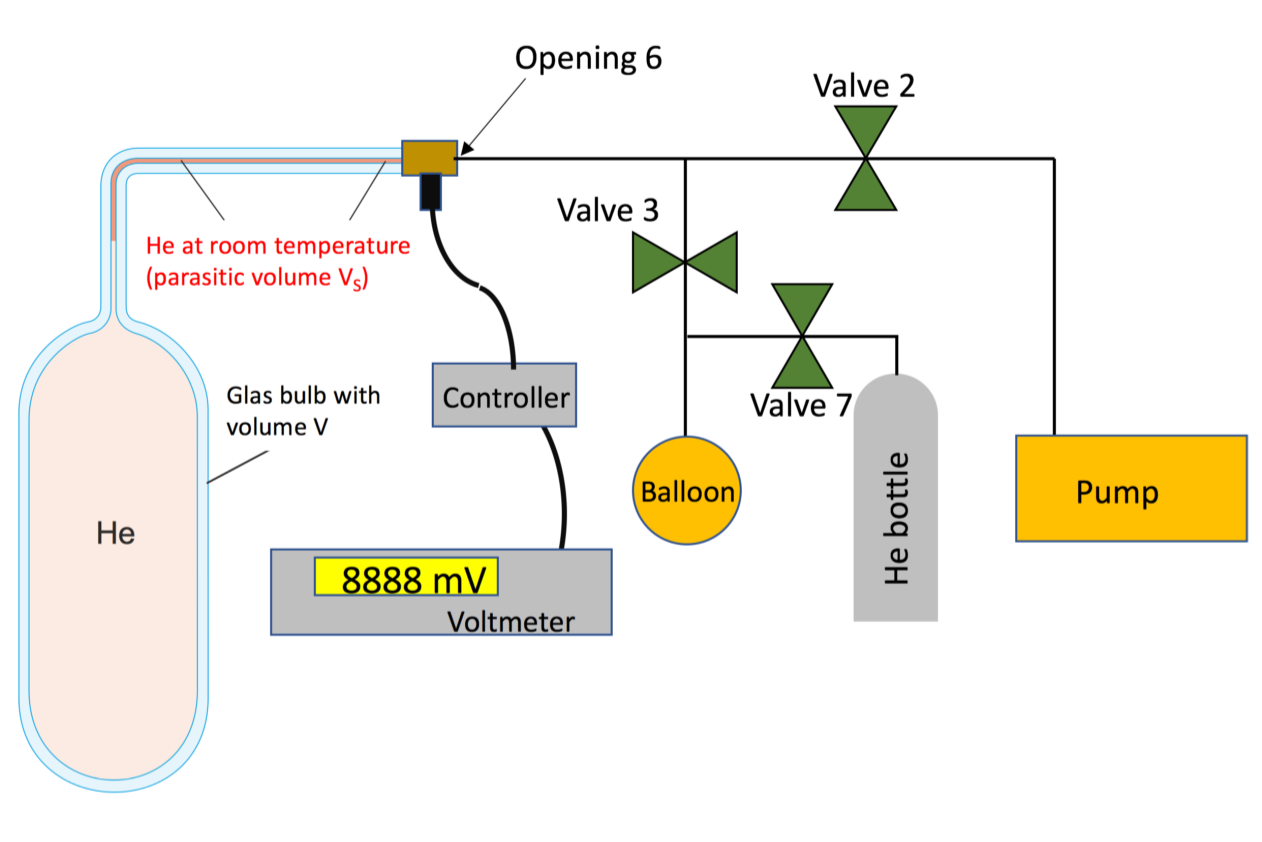
\includegraphics[]{src/images/experimental_setup.png}
        \caption{experimental setup: further explain}
        \label{fig_setup}
    \end{figure}

    Starting with the claibration of the voltmeter, the voltages at room pressure and when a vacuum pump is connected are noted and compared to the actual pressure in the room and the pressure, the pump is able to maintain.
    Hereafter, the glass bulb is evacuated and filled with helium, the reason being that the properties of helium are closer to ideal gases than air.
    Moreover, the oxygen from the air would liquify when cooled down to the temperature of liquid nitrogen (which would happen in the third step of the experiment series) and liquids do not act according to the ideal gas equation.

    In the next step, the helium filled glas bulb is heated to the boiling point of water using steam while leaving the apparatus open so that excess helium can escape.
    We chose the temperature of boiling water as the value can easily be calculated using ambient temperature and pressure as well as tabulated data.
    The gas will only expand in this step and hence no air will get into the glass bulb.
    As soon as the helium has reached the desired temperature, the voltage is taken and the system is closed back up at opening 6. (see Fig.~\ref{fig_setup})
    From now on, the closed system can be used just like a thermometer when calculating the temperature at its corresponding voltage.
    
    To create a linear relation of pressure and temperature in the bulb, a second measurement is needed.
    The temperature at the freezing point of water is also known, so this is the second point used in our case.
    The Helium filled bulb is cooled in an ice bath and the voltage is taken.
    To calculate the absolute zero point of temperature, we have to pay respect to the expansion to the glass bulb with increasing temperature.
    Please refer to section~\ref{sec_results} for the calculation.

    As mentioned before, the closed system acts like a thermometer.
    Therefore, we can cool down the helium filled bulb using liquid nitrogen, read off the voltage and calculate the corresponding temperature of liquid nitrogen.
    In this step, the expansion of the glass bulb must be taken into account too.


\newpage

\section{Results}\label{sec_results}

    In the first step of this experiment, the pressure sensor has to be calibrated at known pressures and temperatures.
    The result of this calibration is presented in Fig.~\ref{fig_calibration}

    \begin{figure}[H]
        \centering
        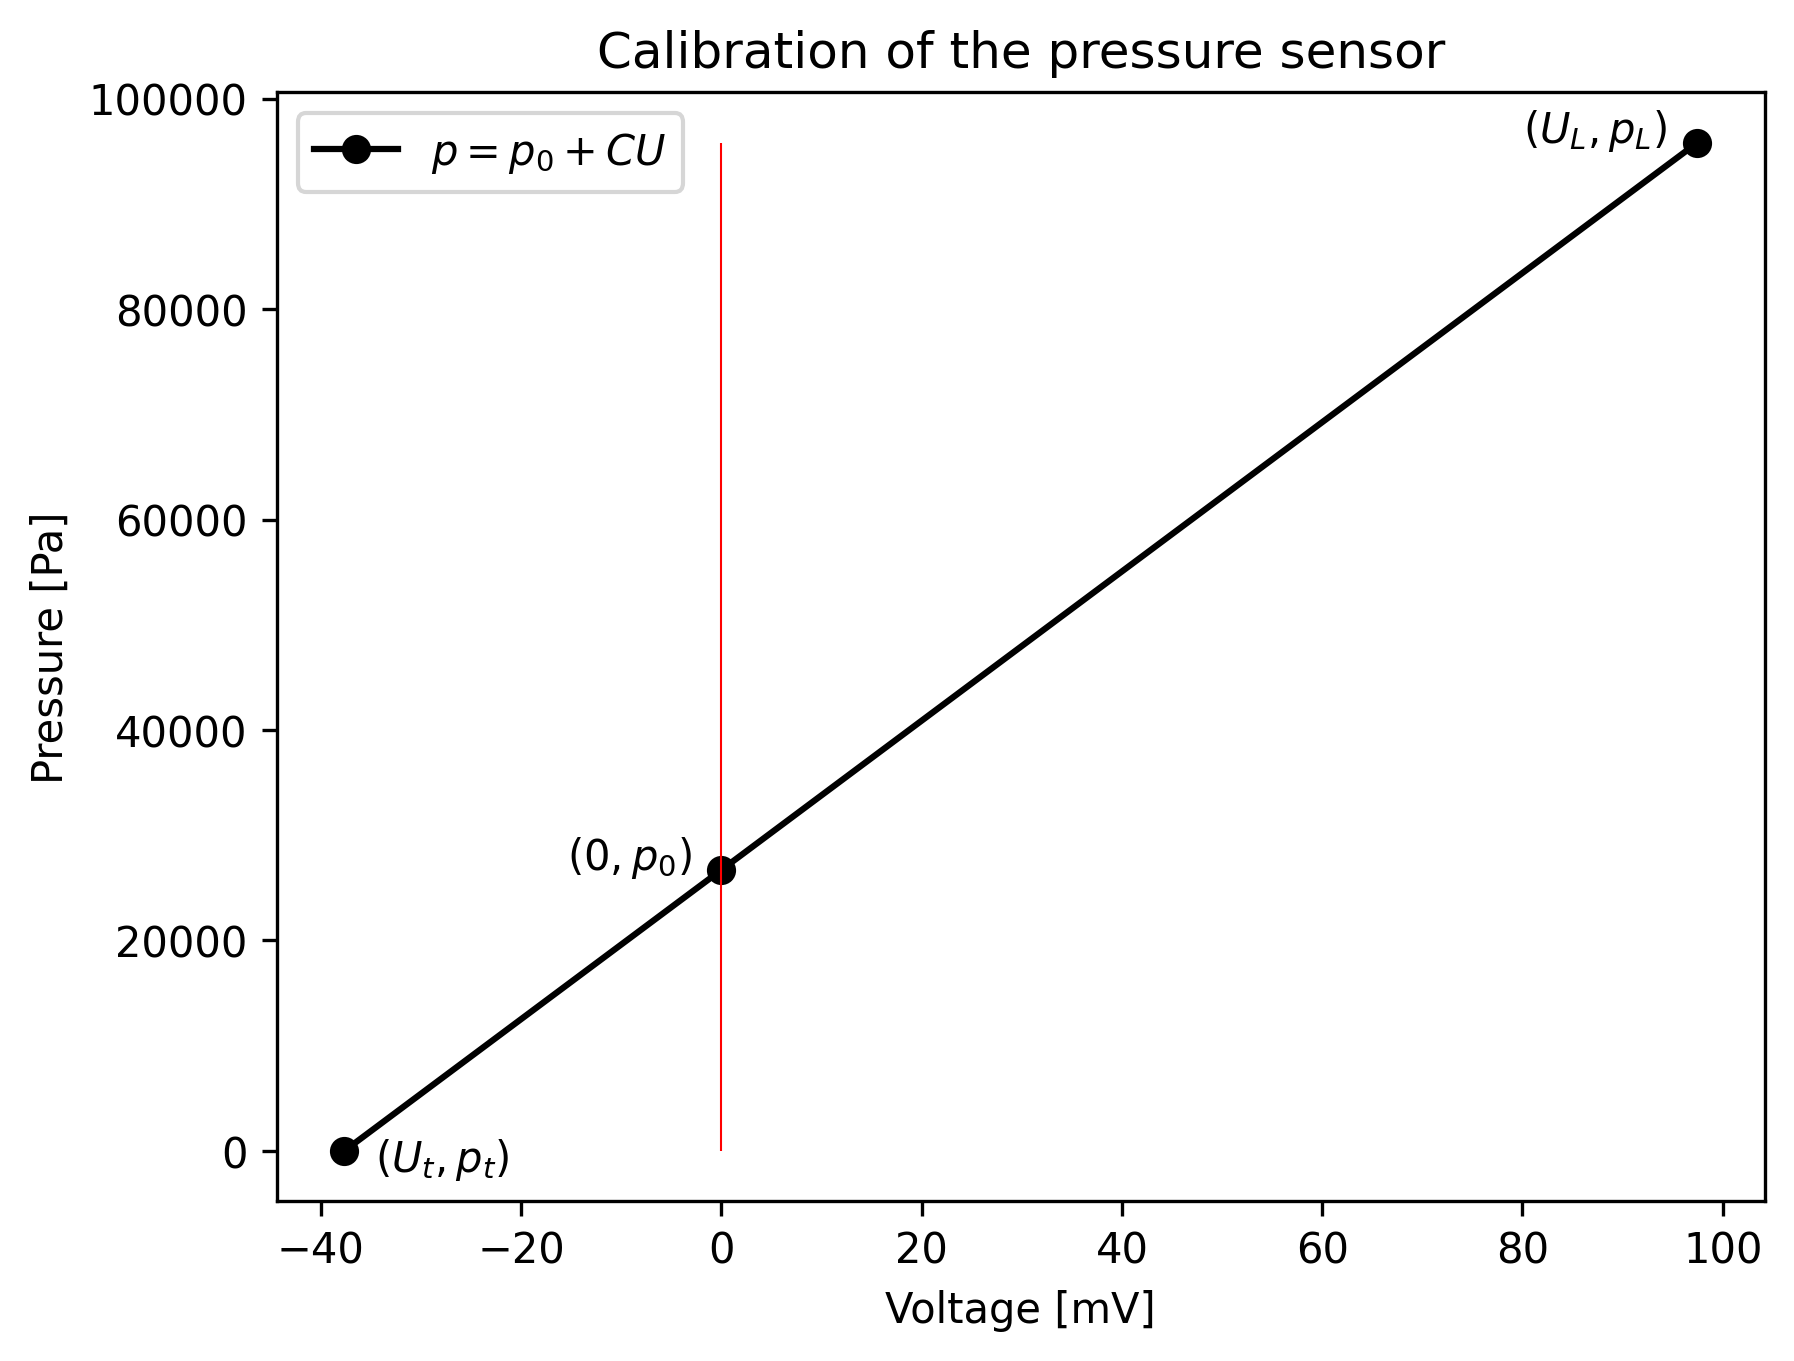
\includegraphics[]{src/images/calibration.png}
        \caption{Calibration of the pressure sensor: A linear fit through $(U_L,p_l)$ and $(U_t,p_t)$ determines the slope $C$. $p_0$ shows the y-intersect at voltage $U_0 = 0$}
        \label{fig_calibration}
    \end{figure}

    $p_0$ can be found by entering a pair of known values into eq.~\ref{eq_pressure}, such as $(U_t,p_t)$.

    \begin{align}
        p_0 = p_t - C U_t \label{eq_p0}
    \end{align}

    Using the slope $C$ and y-offset $p_0$, we determined in this first step, we can calculate the pressure
    of any sensor reading using formula \ref{eq_pressure}.

    \begin{align}
        p(U) = p_0 + CU \label{eq_pressure}
    \end{align}

    To determine the uncertainties in Eq.~\ref{eq_pressure}, we first have to calculate the errors in $p_0$, $C$ and $U$.
    Using the gaussian error propagation, we can then determine the error of the entire equation.


    From the manufacturer's datasheet, we know that the linearity of the sensor is guaranteed up to $\pm 0.05\%$ full scale.
    This means that the sensor signal error is at most $0.05\%$ of $150\si{\milli\volt}$, thus $0.075\si{\milli\volt}$.

    Furthermore, it has to be taken into account, that the temperature of the sensor may vary from when
    it was calibrated and when the measurement was made. We can assume a voltage difference of $\pm 0.08\si{\milli\volt}/\si{\celsius}$ at $p = 0$.
    The slope of this curve can vary by $\pm 0.1\% \si{\celsius}$
    This is the uncertainty calculation for $\Delta U$:
    \begin{align}
        \Delta U &= 0.075 \si{\milli\volt} + 0.08 \frac{\si{\milli\volt}}{1 \si{\celsius} \pm 0.1 \% \si{\celsius}}\\
        &= 0.075 \si{\milli\volt} + 0.08 \si{\milli\volt} + 8 \cdot 10^{-5} \si{\milli\volt} \label{eq_dlta_u}\\
        \bf \Delta U &= \bf \pm 0.15508 ~\si{\bf\milli\volt} \label{dlta_u}
    \end{align}

    The errors in eq.~\ref{eq_dlta_u} were calculated using the gaussian error propagation.

    $\Delta C$ can be determined in a similar way:
    \begin{align}
        C &= \frac{p_L - p_t}{U_L - U_t}\\
        \Delta C &= \sqrt{ \left(\frac{\partial C}{\partial p_L} \Delta p_L \right)^2 +
                        \left(\frac{\partial C}{\partial p_t} \Delta p_t \right)^2 +
                        \left(\frac{\partial C}{\partial U_L} \Delta U_L \right)^2 +
                        \left(\frac{\partial C}{\partial U_t} \Delta U_t \right)^2 } \label{eq_dlta_c}
    \end{align}

    Using the errors for $U$ determined in eq. \ref{dlta_u}, as well as $\Delta p_t = \pm 0.1 \si{\milli\bar}$ given in the manual and $\Delta p_L = \textbf{???}$,
    we can determine a value for $\Delta C$ using eq.~\ref{eq_dlta_c}:
    \begin{align}
        \bf \Delta C = \pm 1.155 \label{dlta_c}
    \end{align}

    Lastly, we have to determine the error for $\Delta p_0$. The error can be calculated in the same way as before, using the equation \ref{eq_p0}.
    \begin{align}
        \Delta p_0 &= \sqrt{ \left(\frac{\partial p_0}{\partial C} \Delta C \right)^2 +
                            \left(\frac{\partial p_0}{\partial U_t} \Delta U_t \right)^2 +
                            \Delta p_t^2}\\
        \bf \Delta p_0 &= \bf \pm 119.001 ~\si{\bf\pascal} \label{dlta_p0}
    \end{align}

    We now have all the values for calculating $\Delta p(U)$. Using eq. \ref{eq_pressure} we can determine the following error propagation:
    \begin{align}
        \Delta p(U) &= \sqrt{ \left(\frac{\partial p}{\partial C} \Delta C \right)^2 +
                            \left(\frac{\partial p}{\partial U} \Delta U \right)^2 +
                            \Delta p_0^2}\\
        &= \sqrt{ \left( U \Delta C \right)^2 +
                \left( C \Delta U \right)^2 + 
                \Delta p_0^2} \label{eq_dlta_p}
    \end{align}

    \begin{figure}[H]
        \centering
        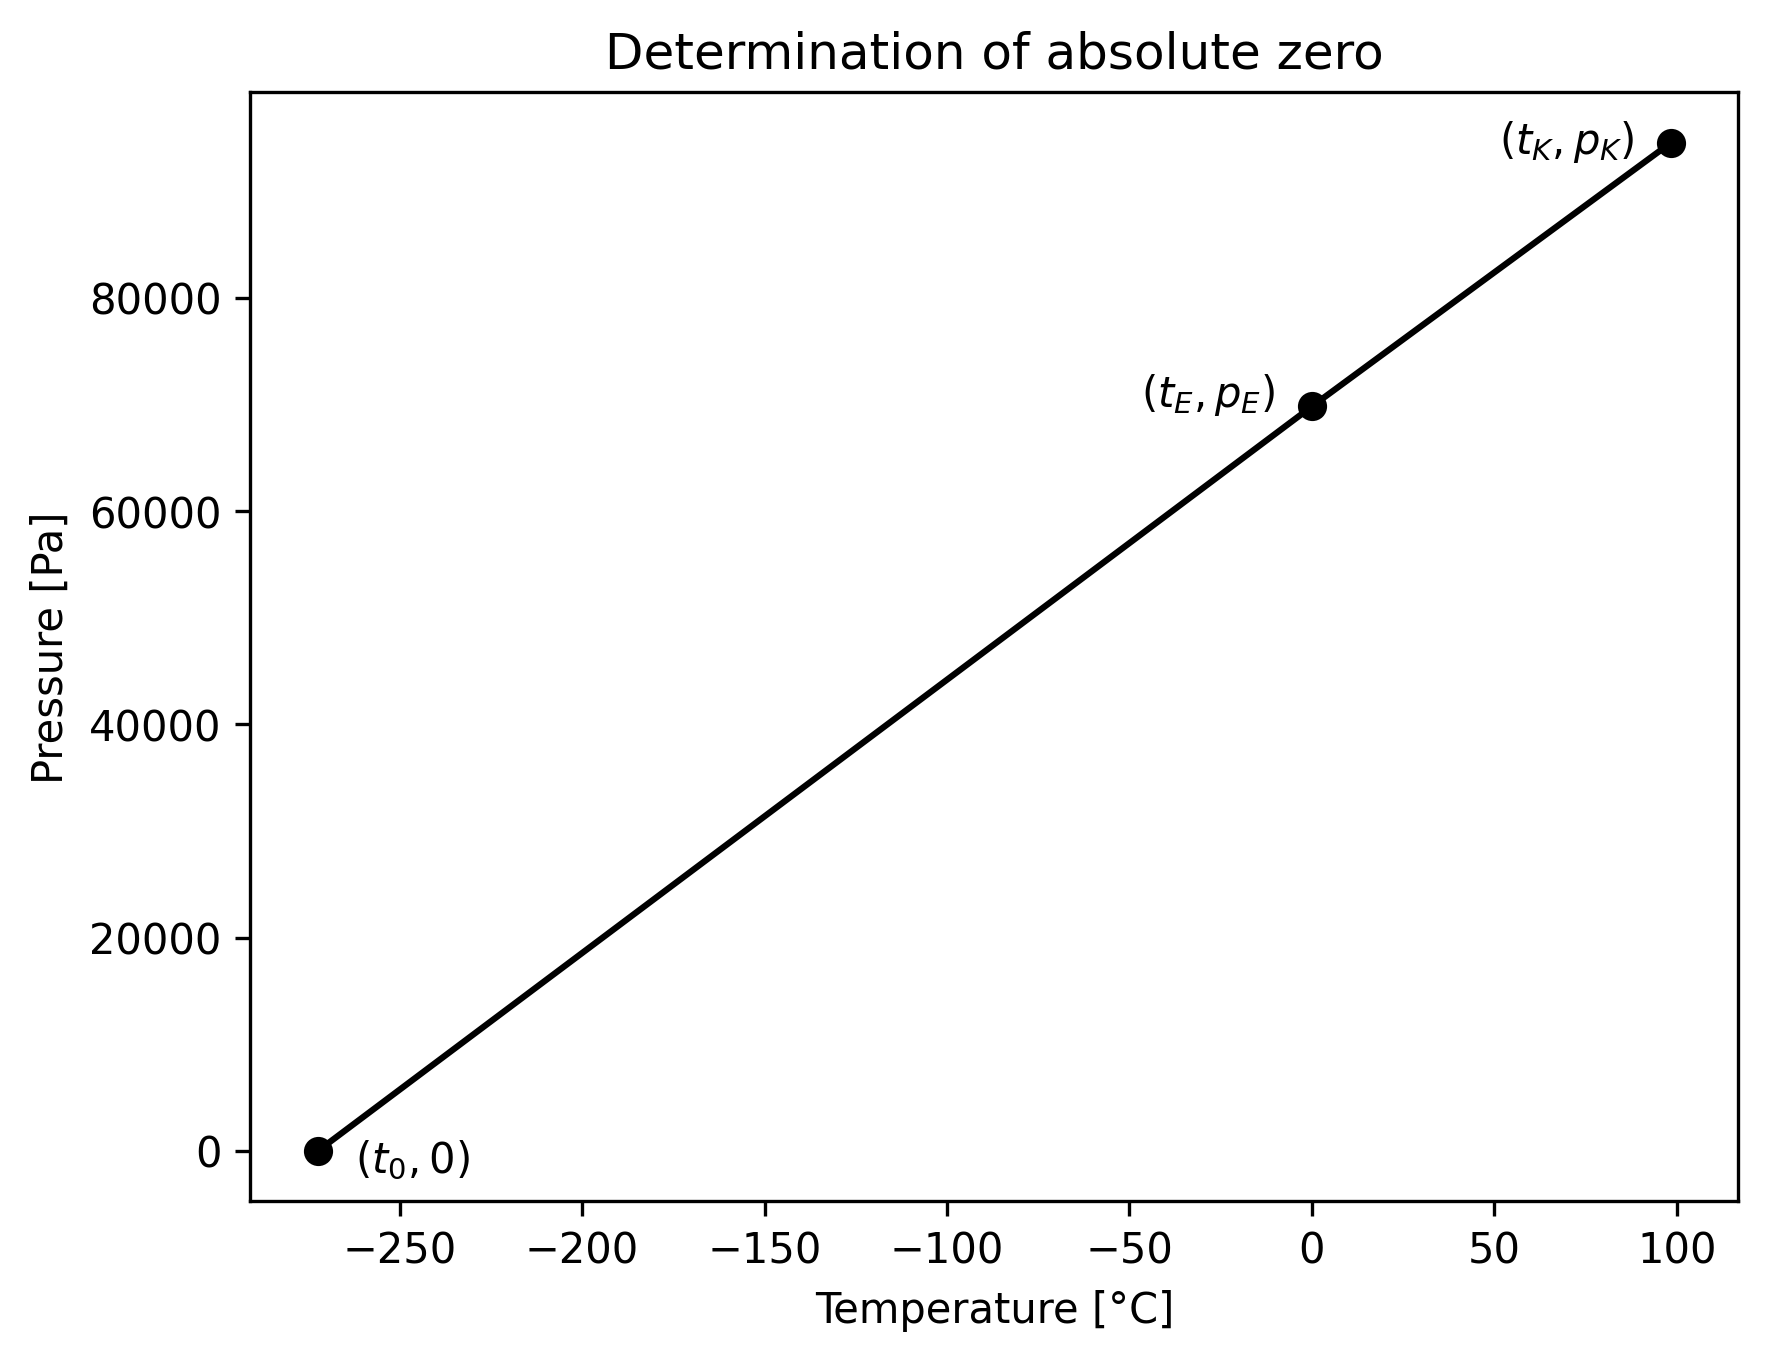
\includegraphics[]{src/images/absolute_zero.png}
        \caption{Determination of absolute zero: Linear fit through $(t_E, p_E)$ and $(t_K, p_K)$ until $p = 0$ is reached.}
        \label{fig_abs_zero}
    \end{figure}

    In this following chapter the results from the determination of absolute zero are presented.
    Using eq.~\ref{eq_pressure} the resulting pressures were calculated from the raw sensor data.
    With the derived eq.~\ref{eq_dlta_p} we can then calculate the errors $\Delta p_K, \Delta p_E$.
    \begin{align}
        p(U_E) &= 69814 ~\si{\pascal}\\
        p(U_K) &= 94535 ~\si{\pascal}\\
        \Delta p_E &= \pm 176.6 ~\si{\pascal} \label{val_pE}\\
        \Delta p_K &= \pm 196.1 ~\si{\pascal} \label{val_pK}
    \end{align}

    As described above the exact value for $t_0$ has to take into account the remaining gas
    in the tube connecting the bulb with the sensor, as well as the thermal expansion of the
    bulb itself. The following quadratic equation calculates the final value for $t_0$ while
    taking into account the factors stated above.
    \begin{align}
        a &= (1 + \varepsilon)p_E - (1 + \epsilon + \gamma t_K)p_K\\
        b &= \varepsilon(p_K - p_E)t_K + (1 + \gamma t_K)p_K t_L - p_E(t_L + t_K)\\
        c &= p_E t_L t_K\\
        t_0 &= \frac{-b \pm \sqrt{b^2 - 4a c}}{2a} \label{eq_t0}
    \end{align}

    Using a barometer in the lab we determined the boiling point of water to be $t_K = 98.323 \si{\celsius}$.
    The temperature in the lab was $t_L = 24 \si{\celsius}$.
    When entering the results from eq.~\ref{val_pE} and~\ref{val_pK}, as well as $t_K$ and $t_L$ into eq.~\ref{eq_t0},
    we get the following result for $t_0$:
    \begin{align}
        t_0 = -272.31~\si{\celsius} \label{val_t0}
    \end{align}

    The error calculation for $t_0$ was again accomplished using the gaussian error propagation.
    Due to the fact that $t_E$, as well as $t_K$, could be determined very precisely, we did not take
    the uncertainties of these values into account in the following error calculation.
    Therefore the only variables with errors are $p_E$, as well as $p_K$.
    \begin{align}
        \Delta t_0 &= \sqrt{ \left(\frac{\partial t_0}{\partial p_E} \Delta p_E \right)^2 +
                            \left(\frac{\partial t_0}{\partial p_K} \Delta p_K \right)^2 }\\
        \Delta t_0 &= \pm 0.4427195~\si{\celsius} \label{dlta_t0}\\
        \bf t_0 &= \bf -272.31 \pm 0.44272~\si{\bf\celsius} \label{res_t0}
    \end{align}

    In the last part of the experiment, the apparatus was used as a thermometer, to determine the 
    temperature of liquid nitrogen.
    Using eq.~\ref{eq_pressure} the pressure $p_N$ was calculated from the raw sensor data $U_N$.
    \begin{align}
        p_N = 19635 \si{\pascal}
    \end{align}

    To calculate the temperature $t_N$ of liquid nitrogen we can use our known value of $t_0$ and solve
    the following equation for $t'_{LN2}$.
    \begin{align}
        \frac{p_E}{t_E - t_0} \approx& \; \frac{p_N}{t'_{LN2} - t_0}\\
        t'_{LN2} \approx& \; \frac{p_N}{p_E}(t_E - t_0) + t_0
    \end{align}

    Here we again have to take the volume of gas in the tube connecting the bulb with sensor,
    as well as the shrinkage of the glass bulb due to the temperature change into account.
    The following equation will give us an exact value for $t_{LN2}$:
    \begin{align}
        A \equiv& \; \frac{p_E}{t_E - t_0} + \frac{\varepsilon(p_E - p_N)}{t_L - t_0}\\
        =& \; 256.54 \textbf{UNITS}\\
        t_{LN2} =& \; \frac{A t_0 + p_N}{A - \gamma p_N}\\
        =& \; -195.92~\si{\celsius} \label{val_tN}
    \end{align}

    Using the gaussian error propagation the uncertainty for $t_{LN2}$ was calculated. As stated above
    the uncertainties for the variables $t_L$ and $t_E$ are not considered in this calculation.
    \begin{align}
        \Delta A =& \; \sqrt{ \left(\frac{\partial A}{\partial p_E} \Delta p_E \right)^2 +
                            \left(\frac{\partial A}{\partial p_N} \Delta p_N \right)^2 +
                            \left(\frac{\partial A}{\partial t_0} \Delta t_0 \right)^2 }\\
        =& \; 0.7715 \textbf{UNITS}\\
        \Delta t_{LN2} =& \; \sqrt{ \left(\frac{\partial t_{LN2}}{\partial A} \Delta A \right)^2 +
                                    \left(\frac{\partial t_{LN2}}{\partial t_0} \Delta t_0 \right)^2 +
                                    \left(\frac{\partial t_{LN2}}{\partial p_N} \Delta p_N \right)^2 }\\
        =& \; 0.805704~\si{\celsius}\\
        \bf t_{LN2} =& \bf -195.92 \pm 0.80570 ~\si{\bf\celsius} \label{res_tN}
    \end{align}

    % Results
    % This paragraph is where you present the results from your
    % experiment. This could be in the form of a table (if only very few
    % parameters where measured) or as a figure. In the text you should
    % essentially describe what can be seen in the figures, i.e. explain
    % your axis and how the dependent variable changes as a function of
    % the independent variable. Discuss trends of the data as well as the
    % magnitude, origin and nature of the experimental uncertainties. Keep
    % in mind that the measurement results are always correct! They might
    % just not be the answer to the question you had in mind.

    % Depending on the experiment the discussion of the results can
    % also be a part of the data analysis section.



    % Data Analysis
    % In the data analysis section you describe the post processing of the
    % data. How did you obtain the data that you plot in the figures? The raw data does not necessarily need
    % to be presented in the report. An important part of this paragraph
    % are the measurement uncertainties. You should provide the
    % uncertainties of all experimental results, i.e. in the form of error
    % bars. Further, you should explain the origin of these uncertainties.

    % All figures or tables that are part of your report have to be
    % referenced somewhere in the text, ideally in order of their
    % appearance (``as shown in Fig.~\ref{fig1}''). Figures have to
    % have axis labels with units and a sensible scale. If more than on
    % data set is plotted you need to provide a legend. This may be a sentence in the caption (``red dots denote data measured with \SI{1}{\milli\volt}, blue crosses were measured with \SI{10}{\milli\volt}''). Make sure to use a consistent style for all referencing and citing. The best method is to use reference commands like those shown here, which also provide clickable links.

    % After you have presented the data you need to interpret it. To this
    % end you want to discuss the theoretical model that describes your
    % data and you will derive model parameters from your measurement data
    % (i.e. by fitting it to the data). There are many way how you can include equations and mathematical terms in your report. The easiest is to write them inside the text like this: $\Gamma =\SI{1.5}{\micro\meter\per\square\second}$. If you need to write a long equation, it is recommended to use e.g. the align environment.
    %     \begin{align}\label{eq:Gamma}
    %         \Gamma = \frac{a}{4\kappa}\times ...
    %     \end{align}
    % Such an equation can be referenced as Eq.~\eqref{eq:Gamma}. Here, you will again elaborate on
    % the confidence interval of the derived values (error propagation).
    % This is an important part of the report and it will be the basis for
    % the next paragraph.

\section{Discussion}
    We have determined the absolute zero temperature to be \textbf{insert value}.
    The literature value of $t_{0, \text{lit}} = -273.15 \si{\celsius}$, found on the website britannica \cite{literature_absolute_zero} is within our error margins.
    To depict one major use of the calculated value, it is possible to determine a scientific temperature scale known as the Kelvin scale.
    It takes the absolute zero temperature as the starting point while maintaining the same step between every value as the Celsius scale, so $0 \si{\kelvin} = -273.15 \si{\celsius}$.
    This leads to $1K = \frac{\Delta_{0, E}(T)}{273.16000...}$ with $\Delta_{0, E}(T)$ being the difference in temperature between the absolute zero and the freezing point of water.
    The derived scale is used in domains like thermodynamics.

    We made use of our value for $t_0$ by determining the temperature of liquid nitrogen and obtained a value of \textbf{insert value}.
    Again, our margins cover the literature value of $t_{LN2, \text{lit}} = -198.79 \si{\celsius}$ found on britannica \cite{literature_liquid_nitrogen}.
    Knowing the temperature of liquid nitrogen can be useful when in need of a coolant for future research.

    When comparing each obtained value with the literature values, one can be satisfied with the results the experimental setup delivers.

    Still, the error margin could be reduced.
    The biggest impact is given by the error of the slope from the linear relation, resulting from uncertainties in pressure and temperature.
    One portion of the uncertainty in pressure is due to the sensor.
    A higher precision sensor would reduce the error of the slope $\Delta C$.
    Moreover, the temperature change could affect the reading of the sensor, as it is close to the bulb.
    On the other hand, the further away the sensor is located from the helium bulb, the longer the glass tube connecting both.
    Within this tube, a portion of the Helium receives a different heat than the bulb leading to unevenly heated gas in the apparatus.
    That means the pressure in our system is not exactly proportional to the applied temperature.
    Also, the steam used to heat the bulb to the boiling point of water cools down on its way from the bottom to the top of the bulb, resulting in an uneven change of volume of the glassware.
    Therefore, the volume the gas takes up does not exactly match the calculated value.

    % So far you have discussed how you have obtained your data and the
    % quantities you derived from it. In this section you should discuss
    % the results in the context of physical laws. Depending on the
    % experiment you want to compare your result and its uncertainty with
    % the literature value. If you want to confirm a physical model that
    % explains a certain phenomenon you want to assess if this model
    % describes the data well within the confidence intervals, or whether
    % a simpler model describes the data just as well.


    
    
   

\section{Conclusion}
    In this experiment series, we determined the absolute zero temperature $t_0 = (-275.9 \pm 2.45)\si{\bf\celsius}$.
    After having calibrated the apparatus, it could be used as a thermometer and the temperature of liquid nitrogen $t_{LN2} = (-198.5 \pm 2.56)\si{\bf\celsius}$ was found.
    The obtained values are close to the literature values, which confirms the experimental setup to be an effective tool to determine $t_0$ and to use as a thermometer.
    It is possible to derive the Kelvin scale, which serves in different scientific domains, from the values measured and calculated in this experiment.
    However, there are ways to reduce the error margin:
    Waiting for the gas in the apparatus as well as the glass bulb to heat up or cool down is essential to getting the correct result.
    At the same time, the longer we wait, the more air could flow through tiny leaks in the connectons of the tubes.
    Better sealing of the apparatus would ensure less air flow, enable more time for the equilibrium to settle and in turn deliver a better precision of the results.
    Furthermore, monitoring the temperature and pressure of the lab close to the glass bulb while taking the measurement would result in higher certainty.
    Also, a material changing its form less than glass would bring the linear plot closer to the real values

    % In the concluding paragraph you summarize the result, with the
    % emphasis on what you have discovered in this work. You can end this
    % with an outlook on future research, i.e. how could the results be
    % improved or what would be a logical follow up experiment.

\section{Appendix}
    


\begin{thebibliography}{99}

\bibitem{literature_absolute_zero}
Encyclop\ae dia Britannica, The Editors of Encyclopaedia Britannica, Adam Augustyn, absolute zero, \href{https://www.britannica.com/science/absolute-zero}{website} (last visited: 2023.04.02)

\bibitem{literature_liquid_nitrogen}
Encyclop\ae dia Britannica, R. Thomas Sanderson, Comparison of nitrogen group elements, \href{https://www.britannica.com/science/nitrogen-group-element/Comparison-of-nitrogen-group-elements}{website} (last visited: 2023.04.02)

\bibitem{Manual}
Manual to experiment 9 Absolute Zero (2022).


\end{thebibliography}

\end{document}